\subsection{Why other patients make better donors: neurophysiology}
\label{sec:neuro}

\paragraph{Stroke desynchronisation is stronger, wider and shifted, not weaker.} Relative to rest, the 24 chronic patients desynchronised more than the 109 healthy participants almost everywhere (Figure~\ref{fig:neuro}a).
\begin{itemize}
  \item In the mu band, patients reached $-17\pct{}$ to $-25\pct{}$ against $-6\pct{}$ to $-17\pct{}$ for healthy participants. The difference was significant at 11 of 14 channels (Holm-corrected Mann--Whitney tests). The exceptions were C3, Cz and CP3, where the healthy focus lies.
  \item In the beta band, the difference was significant at all 14 channels.
  \item Laterality reversed. Healthy desynchronisation was stronger over the hemisphere contralateral to the imagined hand. Patients' was stronger over the contralesional hemisphere: laterality index $+0.11$ versus $-0.10$ in mu and $+0.13$ versus $-0.17$ in beta, both $p < 0.001$.
\end{itemize}
The shift agrees with the contralesional recruitment reported in more impaired patients \citep{mansour2022}, and is what operator O2 imitates. The stronger ipsilesional desynchronisation contradicts the premise of operator O1. Recording system and paradigm also differ between the cohorts and may contribute to the overall difference in magnitude.

\paragraph{Patients' decision directions agree with each other.} In the re-centred tangent space, each patient's imagery-versus-rest direction was closer to the pooled direction of the other patients than to that of the healthy donors (median cosine 0.87 versus 0.78; Wilcoxon $p = 0.0002$; closer for 22 of 24 patients; Figure~\ref{fig:neuro}b). The within-patient split-half reliability, 0.92, is the ceiling: the other patients' direction comes close to what a second half of the patient's own data would give. This is the mechanism behind the pooling result. Re-centring removes each patient's average covariance, and what transfers is the direction. Other patients supply a direction almost as good as more of the patient's own data; healthy donors supply a biased one, and LesionSim did not correct the bias.

\paragraph{Decodability is stable across the study period.} The own decoder's accuracy did not change significantly between the three S3 time points (Figure~\ref{fig:neuro}c): 87.8\pct{} before ($n = 24$), 85.8\pct{} after ($n = 24$), and 85.6\pct{} at follow-up ($n = 19$). The post-minus-pre change was $-2.0$ points ($p = 0.18$) and follow-up minus pre $-2.1$ points (Holm-adjusted $p = 0.11$). Mu desynchronisation over C3 and C4 was also unchanged ($p = 0.46$ and $0.44$). A decoder calibrated in one session therefore faces a stable target in this cohort, and the pooled donor set does not need to be stratified by time point.

\begin{figure}[t]
\centering
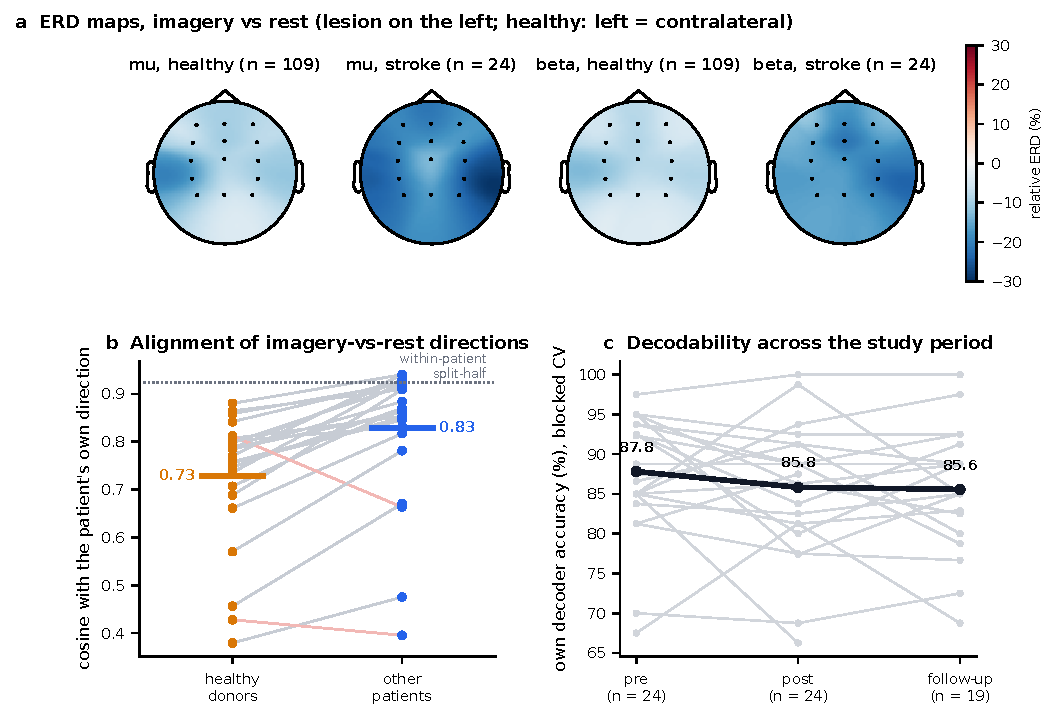
\includegraphics[width=\linewidth]{figures/fig6_neuro.pdf}
\caption{Neurophysiology of S3 (all 24 patients, descriptive; fixed methods). \textbf{a}~Relative desynchronisation during affected-hand imagery versus rest, averaged over participants, with the lesion on the left after harmonisation (for healthy participants, left is contralateral to the imagined right hand). \textbf{b}~Cosine between each patient's imagery-versus-rest direction and the pooled direction of healthy donors or of the other patients; the dotted line is the median within-patient split-half reliability. \textbf{c}~Own-decoder accuracy (blocked cross-validation) at the three time points.}
\label{fig:neuro}
\end{figure}
